\section*{Exercice 189 -- Modélisation}
\setcounter{exo}{0}
%CCMP PSI 2005


Le schéma-bloc global de l’asservissement de l’accélération en phase de traction est représenté figure suivante. 

%\begin{obj}
%\end{obj}

\begin{center}
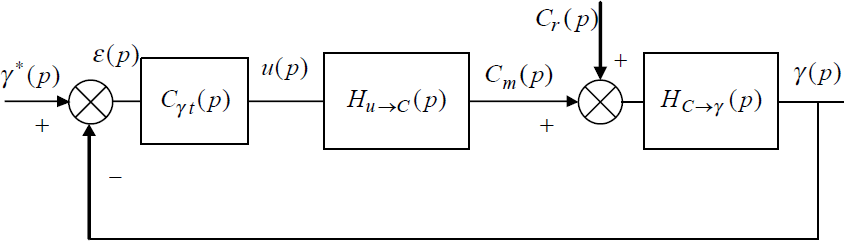
\includegraphics[width=\linewidth]{980_01}%
\end{center}

On adoptera par la suite les fonctions de transfert suivantes : $H_{u\rightarrow C}(p)=\dfrac{40p}{\left( 1+4p\right)\left(1+0,4 p \right)}$ et $H_{C\rightarrow \gamma}(p)=0,00075$.

\subparagraph{}
\textit{La réponse fréquentielle du module et de la phase dans le plan de Bode de la fonction de
transfert en boucle ouverte de la figure précédente pour $C_{\gamma t} ( p) = 300 $  a été reportée ci-dessous.
Analyser les performances du système asservi par $C_{\gamma t} (p) = 300 $ (pulsations de coupure
à \SI{0}{dB} et marges de phase et de gain).}
\ifprof
\begin{corrige}
\end{corrige}
\else
\fi

\begin{center}
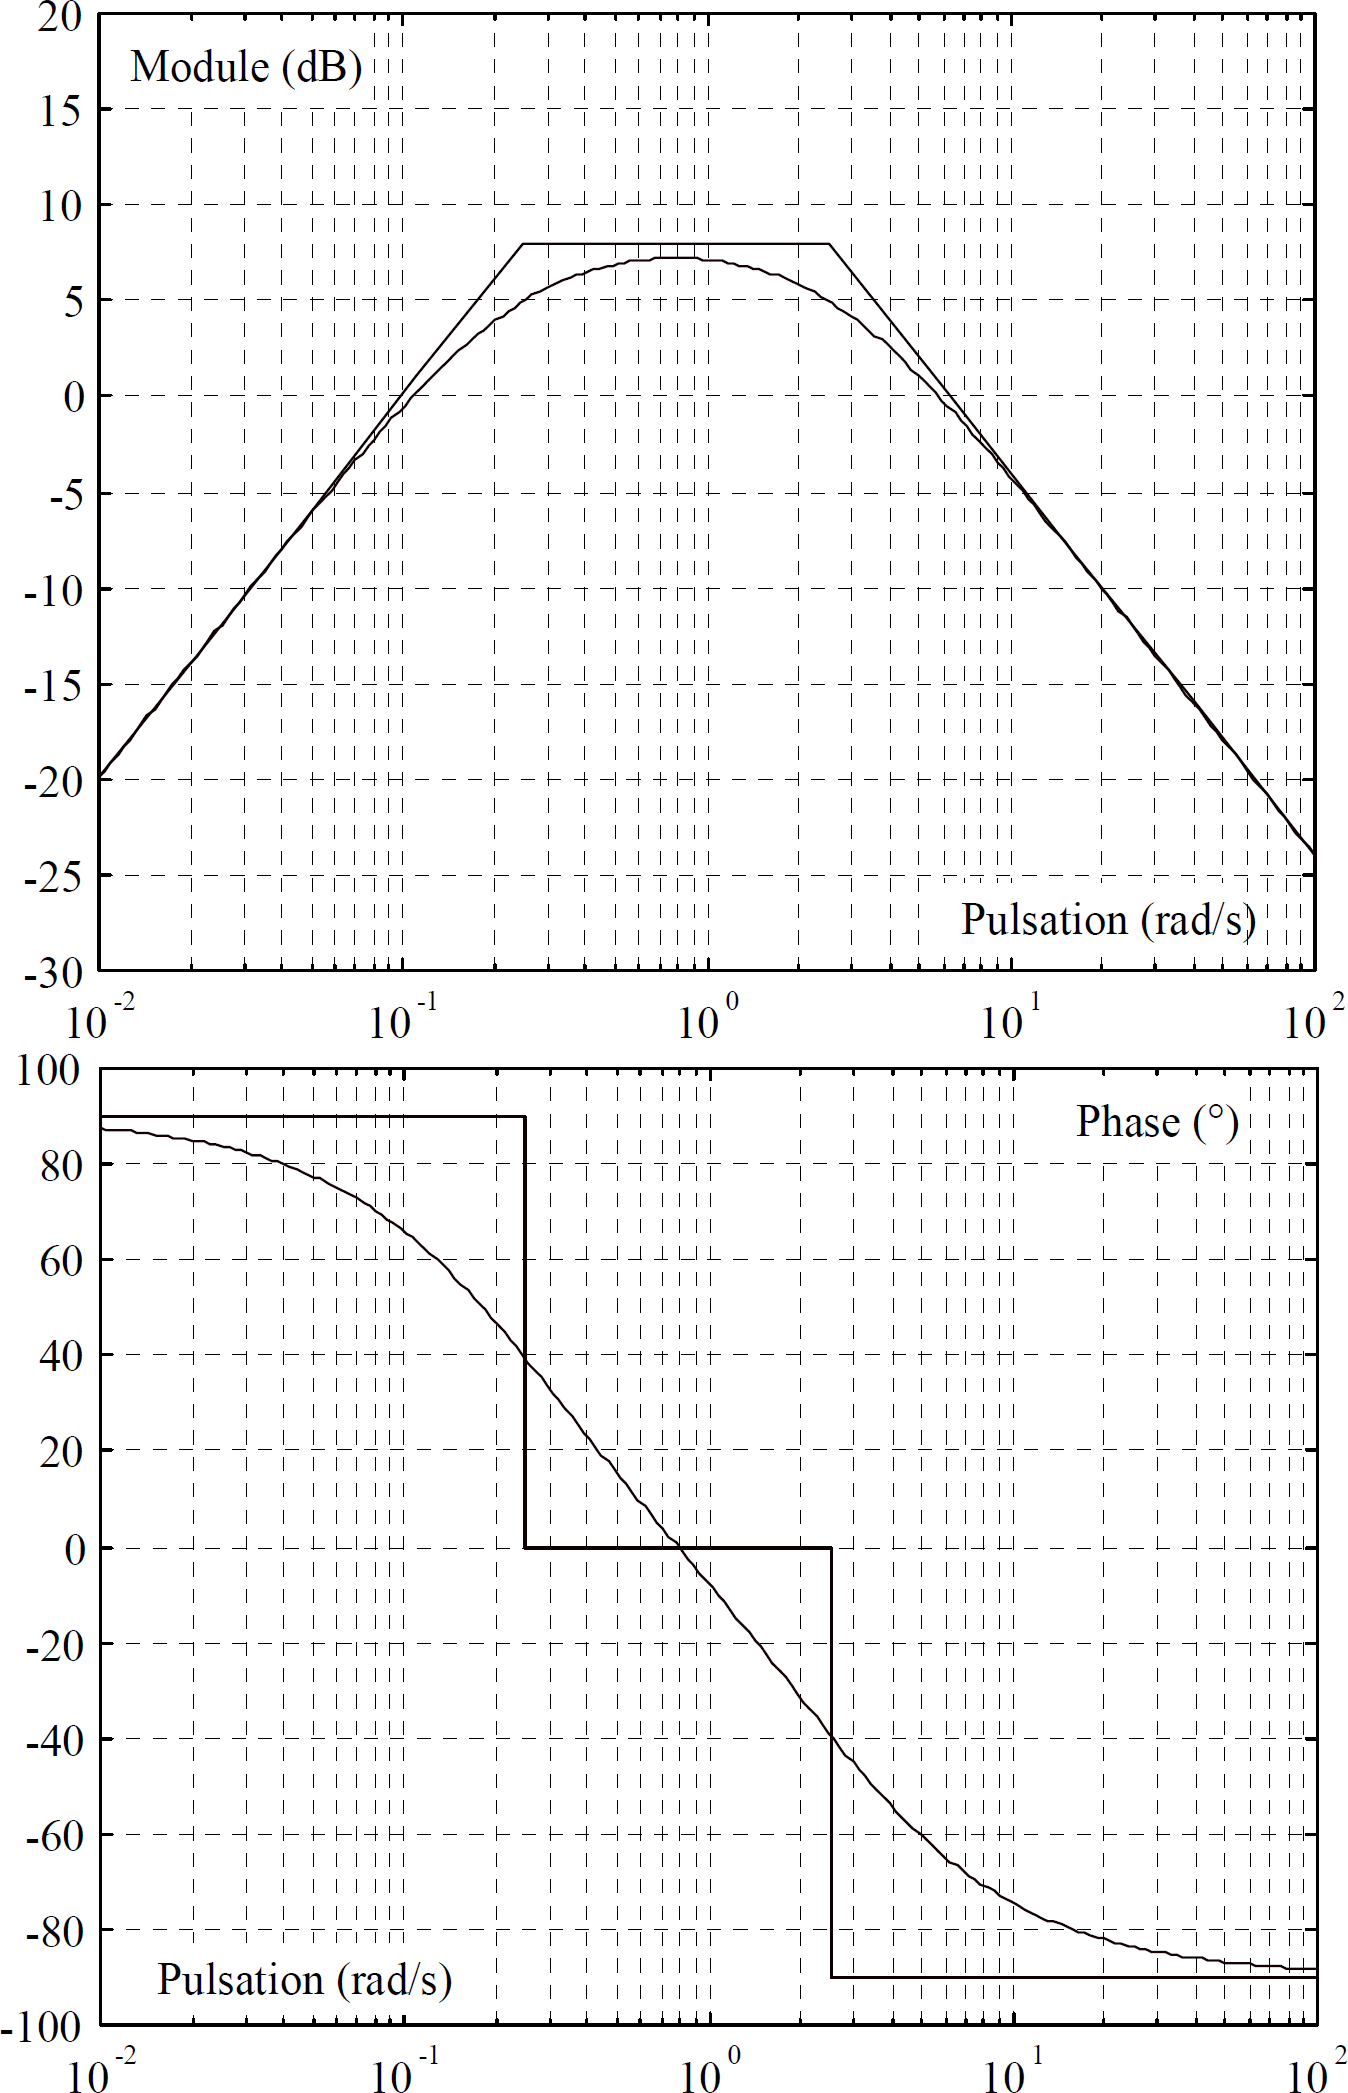
\includegraphics[width=\linewidth]{980_02}%
\end{center}

La réponse $\gamma(t)$ du système asservi par $C_{\gamma t} ( p) = 300$ à un échelon unité d’accélération $\gamma^* (t)$ est reportée figure suivante.

\begin{center}
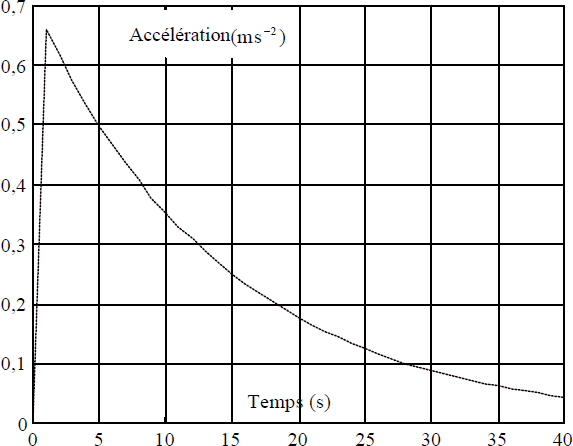
\includegraphics[width=\linewidth]{980_03}%
\end{center}

\subparagraph{}
\textit{Sur le diagramme donnant le module de la fonction de transfert en boucle
ouverte, dessiner en bleu l’allure asymptotique du module de la réponse fréquentielle de la boucle
fermée d’accélération.}
\ifprof
\begin{corrige}
\end{corrige}
\else
\fi

\subparagraph{}
\textit{Justifier alors l’allure de la réponse indicielle de la figure précédente.}
\ifprof
\begin{corrige}
\end{corrige}
\else
\fi

On souhaite conférer au système asservi une pulsation de coupure haute en boucle ouverte à \SI{0}{dB}
$\omega_c = \SI{2}{rad.s^{-1}}$. On corrige la structure bouclée par le correcteur de type Proportionnel Intégral (P.I.) :
$C_{\gamma t}(p)=K\dfrac{1+10p}{10p}$.


\subparagraph{}
\textit{Construire en bleu dans le plan de Bode le module et la phase de la boucle ouverte corrigée incluant le correcteur 
$C_{\gamma t} (p)$ avec $K = 1$. On donne $20 \log( 2) \simeq  6,0$ et$ 20 \log(3) \simeq 9,5$ .}
\ifprof
\begin{corrige}
\end{corrige}
\else
\fi


\begin{center}
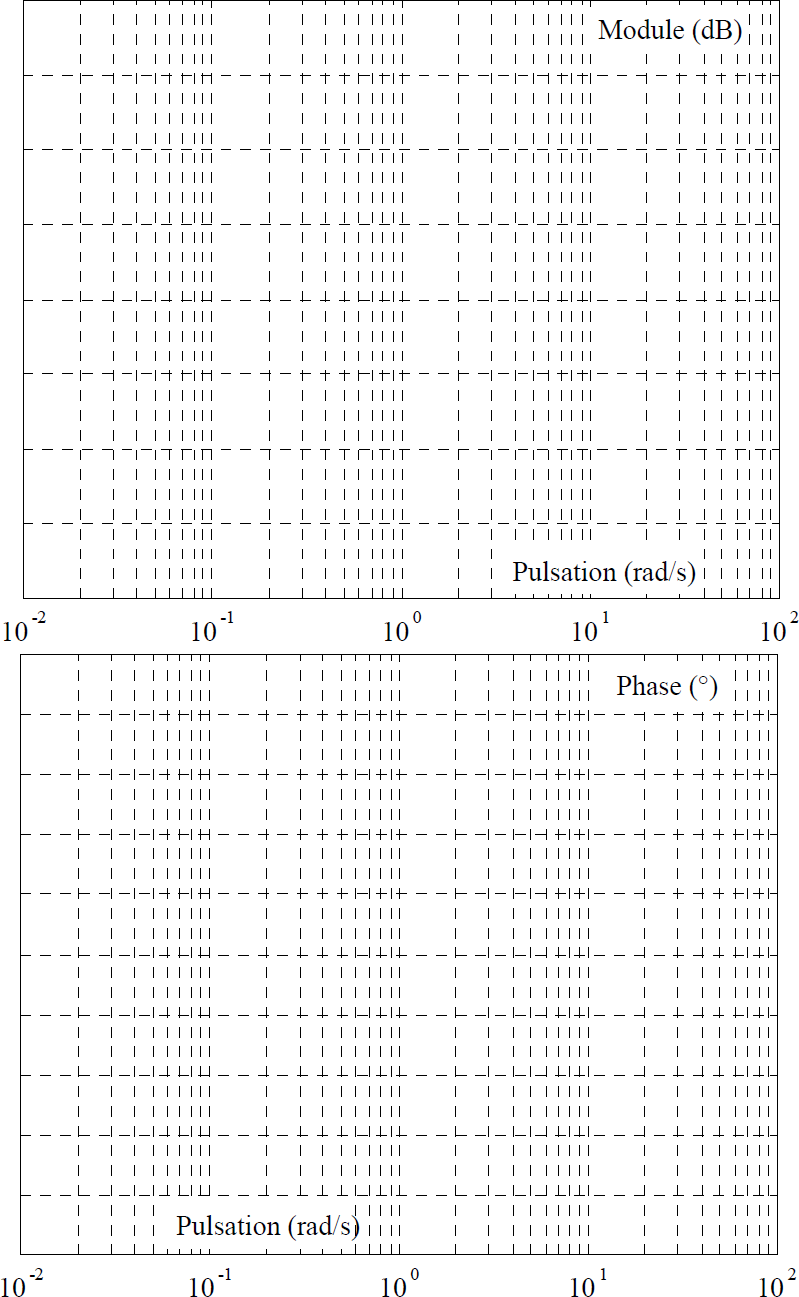
\includegraphics[width=\linewidth]{980_04}%
\end{center}


\subparagraph{}
\textit{Déterminer le gain $K$ de ce correcteur de façon à satisfaire la spécification sur la pulsation de
coupure haute. On donne $10^{2,1}\simeq  126$, $10^{2,2}\simeq  158$, $10^{2,3}\simeq  200$ .}
\ifprof
\begin{corrige}
\end{corrige}
\else
\fi



\subparagraph{}
\textit{En incluant le correcteur $C_{\gamma t} (p)$ déterminé précédemment, calculer l'erreur en régime
permanent pour une entrée $\gamma ^* (t)$ en échelon d’amplitude $\gamma^*_0$ et un couple perturbateur $C_r (t)$ en
échelon d’amplitude $C^*_{r0}$ .}
\ifprof
\begin{corrige}
\end{corrige}
\else
\fi


\subparagraph{}
\textit{Le résultat était-il prévisible dans le cadre de la correction envisagée ? 
Justifier ce résultat par rapport à la forme de la fonction de transfert du système.}
\ifprof
\begin{corrige}
\end{corrige}
\else
\fi

\begin{enumerate}
\item $\omega_{c1} = \SI{0,1}{rad.s^{-1}}$ et $\omega_{c2} = \SI{6}{rad.s^{-1}}$, $MG=+\infty$, $M\varphi = 110\degres$.
\item ...
\item ...
\item ...
\item ...
\item $\varepsilon_{\gamma} = \dfrac{40 K K_{C \gamma}}{10+40 K K_{C \gamma}}\gamma_{0}^*$, 
$\varepsilon_{\text{pert}} = \dfrac{ K_{C \rightarrow \gamma}}{1+4K K_{C \rightarrow \gamma}}C_{r0}^*$.
\item ...
\end{enumerate}